\chapter{Intro}\label{ch:intro}

In recent months and years, neural networks have produced many \textit{state-of-the-art} results in almost all possible disciplines of machine learning. One of the disciplines is Natural Language Processing, \textit{NLP} for short. This term covers many other hot research disciplines, including 

\begin{itemize}
\item Sentiment Analysis
\item Machine Translation
\item Voice Recognition
\item Text Generation
\end{itemize}

Another term for text generation is denoted by \textit{Language Modelling}, because it uses the words and grammar as input for the model. In the last 5 years, there were mainly two approaches for modelling NLP, namely the rule-based system and the template-based system (Figure \ref{rules_based}). Today the \textit{State-of-the-Art} are the neural end-to-end systems, which lead to a far more advanced output. These new systems offer more flexibility and scale with a proportionately better results with less required data, because the complexity and thus the required computing power has increased. However, this fact leads to a complexity problem, because it becomes very difficult to understand the decisions of the neural network. The neural network is basically still a \textit{black box} to a large extent, although it gives surprisingly good results, especially in NLP. Nevertheless, neural network models for text processing are difficult to understand, so nowadays compromises between rule-based systems still have to be made and hybrid systems have to be used. 

\begin{figure}
  \begin{center}
  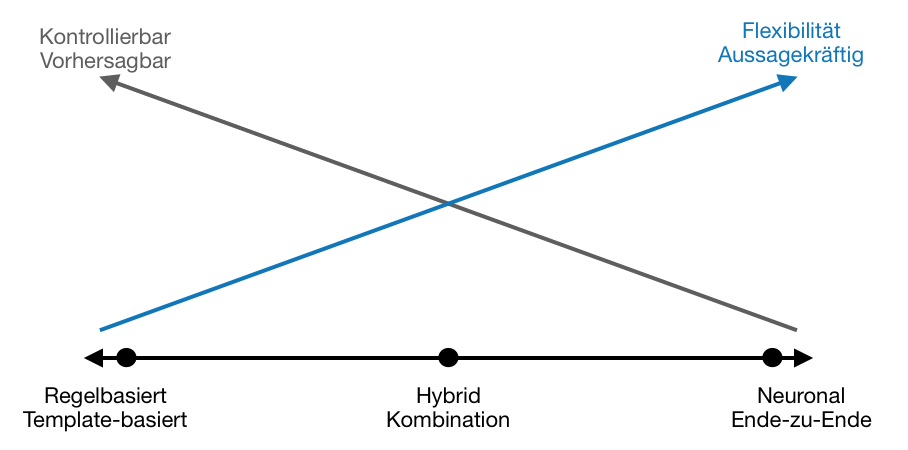
\includegraphics[width=3.5in]{photos/regel_basiert}\\
  \caption{Rule-based- vs. Neural-text-generations-ystem}\label{rules_based}
  \end{center}
\end{figure}

Die natürliche Text Generation, auch \textit{NTG} genannt, hat wiederum viele nützliche und interessante Einsatzgebiete. Darunter zählen  
\begin{itemize}
\item Spracherfassung und Umwandlung in Text
\item Konversationssysteme z.B. Chatbots
\item Textzusammenfassung
\end{itemize} 

Um Sprachmodelle zu trainieren muss ihnen die Wahrscheinlich von auftretenden Wörtern in Abhängigkeit der vorangegangen Wörter beigebracht werden. Es gibt mehrere Ansätze um dieses Ziel zu erreichen. Sprachmodelle können auf Ebene der Wörter, ganzer Sätze oder sogar ganze Paragraphen trainiert werden. Die Granularität in welcher das Training stattfindet wird als \textit{n-grams} bezeichnet, wovon  \textit{n} die Anzahl der vorangegangen Wörter repräsentiert.

\section{Case study of a current NLP system}

\subsection{Case study}

Image-to-Text | Captionbot Microsoft

\subsection{Useful application areas of NLP systems}

IoT, Grammerly, ok

\subsection{Useful application areas of NTG systems}